\section{Разбиения множеств}\label{sec:ch-1-sec-2}


\begin{definition}[Разбиение мн-в]
    $A \neq \varnothing$, тогда $K$ --- \definiendum{разбиение} $A$, если
    $\begin{cases}
         K \subseteq 2^A,\\
         \bigcup K = A,\\
         \forall k, l \in K \Rightarrow k \cap l = \varnothing,\\
         \varnothing \notin K.
    \end{cases}$
\end{definition}

\begin{definition}[Измельчение разбиения]
    $\sqsupset K, L$ --- разбиения $A$, тогда говорят, что $K$ \definiendum{измельчает} $L$, если $\forall ~k \in K ~\exists ~l \in L: k \subseteq l$.
\end{definition}

\begin{definition}[Произведение разбиений]
    $\sqsupset K, L$ --- разбиения $A$, тогда \definiendum{произведение разбиений} --- наибольшее по включению разбиение $A$, измельчающее $K$ и $L$.
\end{definition}

\begin{sh-proposition}
    Произведение разбиений существует.
\end{sh-proposition}

\begin{proof}
    Неформально: смотрим картинку и радуемся жизни

    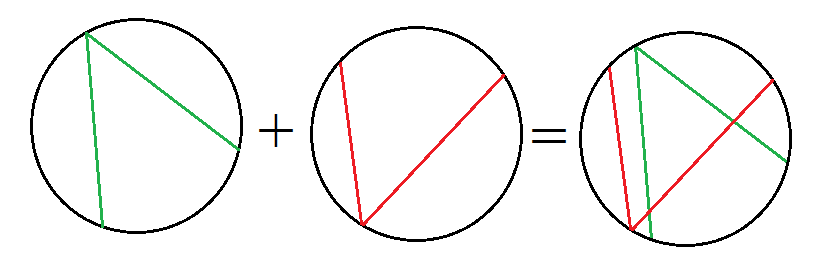
\includegraphics[scale=0.5]{res/произведение разбиений}

    Чуть более формально: пересекаем все $X \in K$ со всеми $Y \in L$ и выкидываем пустые множества, получаем то, что надо.

    Ещё более формально: пусть $B = \{X\cap Y : X\in K, Y\in L, X\cap Y \neq \varnothing\}$.

    $B$ — разбиение $A$, так как $\forall ~b \in B ~b \in 2^A, b \neq \varnothing, \forall ~a \in A ~\exists! ~b\in B: a\in b$.

    Пусть $C$ --- тоже разбиение $A$, измельчающее $K$ и $L$, покажем, что $C$ измельчает и $B$.

    Пусть $c \in C \Rightarrow ~\exists ~X \in K ~\exists ~Y \in L: c\subseteq K$ и $c \subseteq L \Rightarrow c \subseteq K \cap L \Rightarrow ~\exists ~b=K\cap L \in B: c\subseteq b$.

    При желании можно накрутить ещё формализма, но так ли оно надо?
\end{proof}